\section{TEMEL KAVRAMLAR}

\subsection{Band Genişliği (Bandwidth)}
\tab Haberleşme kanalının veya iletim ortamının kapasitesini ifade etmek için kullanılır.
Analog sinayallerde birini \textbf{\textcolor{violet}{hertz (hz)}} iken digital sistemlerde \textbf{\textcolor{violet}{bps (b/s)}}.\\
bir haberleşme sistemi, gönderirici, alıcı ve iletim ortamından oluşur.
İletim kapasitesi en büyük olan bütün sistemin bant genişliği belirler.

\textcolor{red}{Örnek}:
\begin{figure}[ht]
    \centering
    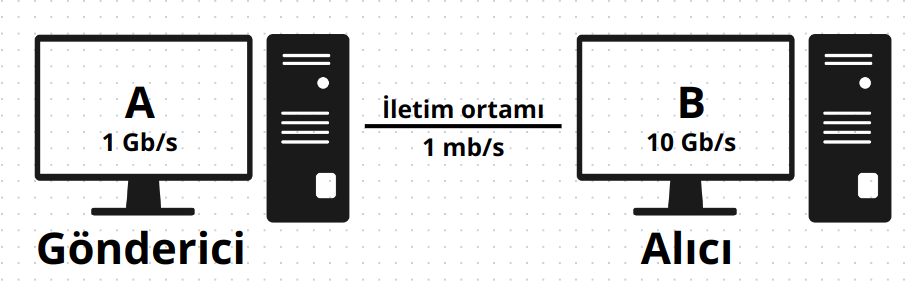
\includegraphics[width=17cm]{images/bandwidth}
    \caption{Bant Genişliği}
    \label{fig:bandwidth_example}
\end{figure}

\textbf{\textcolor{red}{Soru}}
\begin{enumerate}
    \item 240 mb büyüklüğündeki bir MP3 dosyası bir sistemde 4dk'da aktarılıyor.
    Bu sistemin aktarım kapasitesini (bant genişliğini) bulunuz.
    \item MP3 yerine MPG olsaydı ne olurdu?
\end{enumerate}

\textbf{\textcolor{red}{Çözüm}}

Bw=?
\begin{enumerate}
    \item 4dk 240 mb => saniyede 1mb = \textcolor{red}{8mb/s}
    \item Değişim olmaz...
\end{enumerate}

\subsection{Temel Band (Base Band)}
\tab İletim ortamında tek bir frekans bandı kullanılır.
Böylece teorik olarak iletim ortamının tüm kapasitesi tek bir kanal için kullanılır.\\
\textbf{Örneğin}: Ethernette bu band kullanır.

\subsection{Geniş Band (Brood Band)}
\tab İletim ortamında birden fazla frekans bandı kullanılır.
bulunur. Basit bir frekans band filtresi sayesinde kanallar ayrıştırılabilir.
Telefon hattından aynı anda ses verinin taşınması buna örnektir.
\begin{figure}[ht]
    \centering
    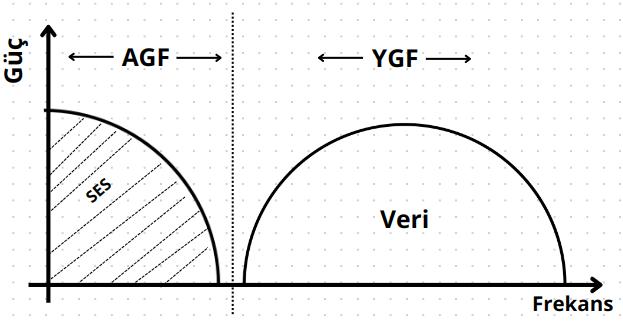
\includegraphics[width=17cm,height=7cm]{images/brood_band}
\end{figure}

\subsection{Paralel ve Seri İletişim}
\tab Paralel iletişimde byte düzenyinde iletişim sağlanır.
İki uç arasında en az 8 tane fiziksel iletim ortamı olmalıdır.
Band genişliği teorik olarak 8 hat daha fazla olduğu düşünülebilir.
Ancak hem maliyet hem protokol tercihi hem de kullanılan topoloji gibi ektenler bu konuda etkilidir.

\subsection{Haberleşme Kanalı Modlari}
\begin{enumerate}[label=\alph*)]
    \item \textbf{\textcolor{blue}{ Simplex Kanal}}: Televizyon ve radyo gibi yayının tek taraflı olarak yapıldığı kanallardır.
    \item  \textbf{\textcolor{blue}{ Half-dubleks Kanal}}: Çıft yönlu iletişim vardır.
    Ancak aynı anda sadece bir taraf veri gönderebilir. Örnek olarak \textbf{\textcolor{red}{telsiz}}.
    \item \textbf{\textcolor{blue}{ Full-dubleks Kanal}}: İki uc arasında iki tane simplex kanal vardır.
    Böylece aynı anda iki taraf veri gönderebilir ve alabilir.
    Örnek telefon görüşmeleri.
    \item [!] Günümüzde tüm bilgisayar ağları \textbf{\textcolor{red}{Full-dubleks}}'dir.
\end{enumerate}


